% -*- TeX -*- -*- FR -*-
\documentclass[francais,letterpaper]{uds-article}

%-----------------------------------------------------------------------------
%----- Identification des packages n�cessaires
%-----------------------------------------------------------------------------

\usepackage{babel}
\usepackage[latin1]{inputenc}
\usepackage{color}
%\usepackage{udstitle,dfd}
%\newcommand{\diamant}{Diamant}
\setlength{\oddsidemargin}{0.25in}
\setlength{\evensidemargin}{0.25in}
\setlength{\textwidth}{6.0in}
%\setlength{\parskip}{0.2in}
\newcounter{auxcounter}
\renewcommand{\baselinestretch}{1.5}
\setlength{\parskip}{1.5ex plus0.5ex minus0ex}

\newcommand{\ints}{\renewcommand{\baselinestretch}{1.0}\small \normalsize}
\newcommand{\intm}{\renewcommand{\baselinestretch}{1.5}\small \normalsize}
\newcommand{\intd}{\renewcommand{\baselinestretch}{2.0}\small \normalsize}
\newcommand{\todo}[1]{\textcolor[rgb]{1.00,0.00,0.00}{(TODO: #1)}}

\newcommand{\bi}{\begin{itemize}}
\newcommand{\ei}{\end{itemize}}
\newcommand{\be}{\begin{enumerate}}
\newcommand{\ee}{\end{enumerate}}
\newcommand{\bd}{\begin{description}}
\newcommand{\ed}{\end{description}}



\newcommand{\bv}{\verb}

\newcommand{\bve}{\verb*}

\newcommand{\brun}{\noindent $\triangleright$}
\newcommand{\erun}{$\triangleleft$}

\newcommand{\ang}{\textsf}
\newcommand{\key}{\textsf}
\newcommand{\ita}{\textit}
\newcommand{\bld}{\textbf}
\newcommand{\dos}{\textsc}
\newcommand{\pro}{\texttt}

\newcommand{\diamant}{DIAMANT}
\newcommand{\dia}{DIAMANT 1.0}
\newcommand{\dx}{DIAMANT 1.5}
\newcommand{\saphir}{SAPHIR}
\newcommand{\sig}{SIG}

%% commandes pour les corrections du document
\usepackage{color}
\usepackage{ulem}
\newcommand{\corryannick}[1]{\textcolor[rgb]{1.00,0.00,0.00}{(Yannick: #1)}}
\newcommand{\corrlulu}[1]{\textcolor[rgb]{0.00,1.00,0.00}{(Kader: #1)}}
\newcommand{\corrpascal}[1]{\textcolor[rgb]{0.00,0.00,1.00}{(Olivier: #1)}}
\newcommand{\corrrgr}[1]{\textcolor[rgb]{0.00,1.00,1.00}{(Ruben: #1)}}


%-----------------------------------------------------------------------------
%----- Page Titre
%-----------------------------------------------------------------------------

\Titre{\textbf{- \diamant{} -} \\ \\
SOFTWARE REQUIREMENTS SPECIFICATION\\
\small{\emph{IEEE SRS standard 830-1998}}\\
} \Logo{Images/logoDiamantNew.eps} \Auteurs{Yannick Syam}
\Date{\today}

%-----------------------------------------------------------------------------
%----- Identification des fichiers des pages pr�liminaires et bibliographique
%-----------------------------------------------------------------------------

\FichierResume{}
\FichierRemerciements{}
\FichierGlossaire{} % \FichierLexique est �quivalent
\FichiersBibliographie{udsplain}{}

%-----------------------------------------------------------------------------
%----- Le document
%-----------------------------------------------------------------------------

\includeonly{SRS/historique,SRS/intro, SRS/desc_glob, SRS/func_syst, SRS/req_inter, SRS/req_non_funct, SRS/other_req}

\begin{document}
\begin{articleDX}

%\chapter{Description de la structure de donn�es de \diamant{}}

Le noeud principal de la structure de donn�es de \diamant{} est repr�sent� par la classe \emph{LoadData} (voir figure \ref{datastruct}). Cette classe contient la liste des diff�rentes ressources, � savoir:

\begin{itemize}
    \item \emph{StudentsList} (voir figure \ref{datastruct}): elle repr�sente la structure de donn�es contenant la liste des �tudiants.\\
    \item \emph{RoomsList} (voir figure \ref{datastruct}): elle repr�sente la structure de donn�es contenant la liste des locaux.\\
    \item \emph{InstructorsList} (voir figure \ref{datastruct}): elle repr�sente la structure de donn�es contenant la liste d'instructeurs.\\
    \item \emph{ActivitiesList} (voir figure \ref{datastruct}): elle repr�sente la structure de donn�es contenant la liste d'activit�s.\\
\end{itemize}

Chacune des listes de ressources cit�es ci-dessus h�rite de la super classe \emph{ResourceList}. \emph{ResourceList} contient la liste de tous les �l�ments d'une ressource. Cette liste d'�l�ments est en r�alit� une liste d'objects de type \emph{Resource}. L'object \emph{Resource} d�crit quand � lui un �l�ment par sa cl� (\emph{resourceKey}), son identifiant (\emph{resourceID}) et la nature de cet object (\emph{resourceObject}). Il est � noter que \emph{resourceObject} peut �tre de type \emph{Instructor} ou \emph{Activity} ou \emph{Room} ou encore \emph{Student}

Nous d�crirons chacune des structures dans les prochaines sections.

\begin{figure}[h]
  % Requires \usepackage{graphicx}
  \begin{center}
    \includegraphics[width=430pt]{Images/loaddata.eps}
    \caption{Structure de donn�es}\label{datastruct}
  \end{center}
\end{figure}


\section{\emph{LoadData}}
Cette classe est charg�e de la gestion de deux taches principales
:
\begin{enumerate}
    \item \textbf{Le chargement de fichiers} :  Dans cette �tape, l'int�grit� des fichier des ressources est d'abord v�rifi�e et ensuite chaque fichier est charg� dans un vecteur de bytes pour leur post�rieur
    traitement. Cette t�che est effectu� � l'aide de la classe \emph{FilterFile} de la librairie
    \emph{com.iLib.gIO.FilterFile}.
    \item \textbf{La cr�ation des listes de ressources} : Dans cette �tape chaque liste de ressources est cr��e et peupl�e
    (remplie) avec les �l�ments correspondantes. Cette t�che est
    effectu�e en utilisant les classe d�crites � continuation.
\end{enumerate}

\section{\emph{ResourceList}}
Cette classe impl�mente la structure de donn�es
\emph{ResourceList}.  Elle d�clare les m�thodes
\emph{analyseTokens()} et \emph{buildResourceList()} qui
permettent de peupler la liste du ressource. Cette classe d�finie
les m�thodes n�cessaires pour ins�rer, �liminer, �diter, chercher
et trier les ressources.

\section{\emph{***List}}
Cet ensemble repr�sente les classes \emph{RoomsList},
\emph{InstructorsList}, \emph{ActivitiesList},
\emph{StudentsList}.  Ces classes h�ritent de la super classe
\emph{ResourceList} et, par cons�quent, elles impl�mentent les
m�thodes \emph{analyseTokens()} et \emph{buildResourceList()}.

Comme un cas sp�cial, la classe \emph{StudentsList} a son propre
impl�mentation des m�thodes \emph{removeStudent} et
\emph{removeStudent} car dans ce cas, il faut valider l'existence
de courses de choix de l'�tudiant avant d'ins�rer un nouveau
ressource � la liste et l'existence . \textbf{(V�rifier cette
phrase avec Yannick, pour quoi removeStudent??)}.

\section{\emph{Resource}}
Cette classe impl�mente la structure de donn�es \emph{Resource}.
Elle d�finie les m�thodes n�cessaires pour ins�rer, �diter et
obtenir les champs de la ressource.

\section{\emph{Instructor}}
Cette classe repr�sente la disponibilit� d'un instructeur
appartenant au fichier d'instructeurs (Voir section 1.2). Elle
impl�mente les m�thodes pour g�rer (ins�rer, �liminer, �diter,
obtenir) la disponibilit� d'un instructeur.

\section{\emph{Room}}
Cette classe repr�sente l'information d'un local appartenant au
fichier de locaux (Voir section 1.4).  Elle impl�mente les
m�thodes pour g�rer (ins�rer, �liminer, �diter, obtenir) les
diff�rents propri�t�s d'un local, cela inclut sa disponibilit�.

\section{\emph{Student}}
Cette classe repr�sente l'information d'un �tudiant appartenant au
fichier d'�tudiants (Voir section 1.1).  Elle impl�mente les
m�thodes pour g�rer (ins�rer, �liminer, �diter, obtenir) les
diff�rents propri�t�s d'un �tudiant, cela inclut se choix de
cours.

\section{\emph{Activity}}
Cette classe repr�sente l'information d'une activit� appartenant
au fichier d'activit�s (Voir section 1.3).  Elle impl�mente les
m�thodes pour g�rer (ins�rer, �liminer, �diter, obtenir) les
diff�rents propri�t�s d'une activit�, cela inclut ....\textbf(�
finir)

\chapter*{Historique du document}

% Ce chapitre ne pas obligatoire pour la norme IEEE.
% L'�quipe EXit a d�cid� d'ajouter un fichier historique des changements
% faits sur le document SDD particuli�re de chaque projet.

\begin{tabular}{|p{4.5cm}|p{3cm}|p{7.5cm}|}
  \hline
\textbf{Date} & \textbf{Responsable} & \textbf{Description} \\
  \hline
  10 f�vrier 2005 & Nom  & Premier brouillon.  \\
 \hline
  14 Novembre 2005 & Kader  &  \corrkad{Revision}  \\
  \hline
\end{tabular}


%\part{Architecture}
\chapter{Introduction}


    \section{But}

    \diamant{} est un logiciel servant � la construction d'horaires de
    cours et d'examens sur plusieurs sites � partir d'une interface
    utilisateur.

    \section{Conventions propres � ce document}

    Les anglicismes devront �tre en italique.

    \section{Auditoire cibl� et suggestions de lecture}

    Ce document s'adresse � toutes les personnes impliqu�es dans le
    d�veloppement de \diamant{} tout au long de son cycle de vie: il
    s'agit des utilisateurs, des analystes, des architectes, des
    concepteurs, des testeurs et du chef de projet.

    \section{�tendu du projet}

    \diamant{} est un logiciel de construction d'horaires pr�sent� aux
    utilisateurs sous forme de fen�tre avec une barre de menus,
    contenant des sous-menus. La fen�tre principale pr�sente une
    grille d�crivant l'horaire sur lequel l'utilisateur travaille. En
    dessous de la grille horaire se trouve une barre de t�ches
    \corrpascal{Est-ce une barre de ``t�che'' ou une barre de
    ``statut'' ?}  montrant les ressources en utilisation (�tudiants,
    enseignants, activit�s et locaux) et les conflits d�tect�s.

    Les sous-menus sont de deux types~: ceux qui d�clenchent
    l'ex�cution d'une fonctionnalit� et ceux qui appellent une bo�te
    de dialogue, puis d�clenchent des actions. En g�n�ral ces menus
    entra�nent une mise � jour des donn�es en fonction du traitement
    d�clench�.


    \section{R�f�rences}

    Manuel d'utilisation de \diamant{}. 
\chapter{Description globale}

    \section{Perspective du produit}

    \diamant{} a �t� d�velopp� pour remplacer le logiciel de construction d'horaire \saphir{}, lui m�me d�velopp� sous environ DOS et pr�sentant les principaux d�fauts suivants:
\begin{itemize}
    \item Interfaces peu intuitives et donc pas tr�s facile d'utilisation,
    \item Fonctionnalit�s limit�es, r�duisant ainsi les possibilit�s de l'utilisateur,
    \item Aucune portabilit�,
    \item Difficult� d'adaptation du logiciel au changement des sp�cification,
    \item ...
\end{itemize}

    \section{Fonctionnalit�s du produit}


\subsection{Fonctionnalit� horaire d'examens}
Cette fonctionnalit� est en r�alit� un ensemble de fonctionnalit�s
n�cessaires � la construction d'un horaire des examens. Elle est
d�crite dans le manuel utilisateur.

\subsection{Fonctionnalit� horaire de cours}
Cette fonctionnalit� est en r�alit� un ensemble de fonctionnalit�s
n�cessaires � la construction d'un horaire de cours pour un seul cycle et cet horaire sera ensuite r�p�t� aux autres cycles d'un trimestre (Exp: pour construire l'horaire d'un trimestre comportant 13 semaines de cours, on construit l'horaire d'une semaine de 5 ou 6 jours et cet horaire reste le m�me durant les 13 semaines). Elle est
d�crite dans le manuel utilisateur.

\subsection{Fonctionnalit� horaire trimestriel}

� venir ...

\subsection{Fonctionnalit� affectation d'enseignants}
Cette fonctionnalit� doit servir � assigner � une activit� $n$
enseignants. On peut ajouter uniquement des enseignants qui
sont connus par \diamant{}, c'est-�-dire ceux qui sont dans les fichiers d'importation.

\subsection{Fonctionnalit� modification de la disponibilit� des enseignants}
Cette fonctionnalit� doit permettre de modifier la disponibilit� d'un enseignant (rendre un enseignant disponible ou indisponible dans une p�riode donn�e). Cette modification ne peut se faire que sur des enseignants connus par \diamant{}.

\subsection{Fonctionnalit� manipulation des groupes d'�tudiants}
Cette fonctionnalit� doit permettre de d�placer les �tudiants d'un groupe vers un autre ou encore de ne pas le placer dans un groupe, de figer un �tudiant dans un groupe afin qu'il ne puisse pas �tre d�plac� par le logiciel.

\subsection{Fonctionnalit� Grille partielle}
La fonctionnalit� Grille partielle doit permettre de d�finir et
sauvegarder des  ensembles d'activit�s. Ensuite afficher sur la
grille uniquement les cours de l'ensemble choisi.

\subsection{Fonctionnalit� Importation s�lective}
La fonctionnalit� importation s�lective est de pouvoir importer un
fichier sans changer les donn�es dans les autres fichiers.

\subsection{Fonctionnalit�  Menus}
Les menus doivent �tre disponibles (enabled) ou non disponibles
(disabled) en fonction de la derni�re op�ration effectu� et de
l'�tat du logiciel.

\subsection{Fonctionnalit�  Toolbar}
La fonctionnalit� Toolbar doit permettre d'effectuer, en mode
grille, des modifications (ajout ou suppression de jours,
modification de la priorit� d'une p�riode, modification du nom
d'une journ�e, etc) sur une grille horaire.


\subsection{Fonctionnalit� horaire sans �tudiants}

La fonctionnalit� permet de faire un horaire sans ternir compte du
fichier d'�tudiants, mais uniquement du nombre d'�tudiants associ�
� une activit� (dans le fichier d'activit�).

\subsection{Fonctionnalit� affectation de locaux}

La fonctionnalit� permet d'assigner des locaux aux �v�nements avec
une utilisation optimale des locaux. Les principaux �l�ments �
prendre en compte dans cette affectation sont les suivantes:
\begin{itemize}
    \item La cat�gorie du local a assigner � une activit�.
    \item 
    \item 
\end{itemize}


    \section{Classes et caract�ristiques d'utilisateurs}

    Les principaux utilisateurs de \diamant{} sont: les pr�pos�s
    aux horaires, les s�cr�taires acad�miques, les responsables de
    programmes, les enseignants.

    \section{Environnement d'op�ration (``Operating Environment'')}

    \diamant{} fonctionne sur toutes les plateformes mat�rielles
    et logicielles � condition qu'y soit install� la machine
    virtuelle Java.

    \section{Contraintes de design et d'impl�mentation}

    Describe any factors that will restrict the options available to
    the developers and the rationale for each constraint. Constraints
    might include the following:

    \begin{itemize}
        \item Specific technologies, tools, programming languages, and
              databases that must be used or avoided.
        \item Restrictions because of the product's operating
              environment, such as the types and versions of Web
              browsers that will be used.
        \item Required development conventions or standards. (For
              instance, if the customer's organization will be
              maintaining the software, the organization might specify
              design notations and coding standards that a
              subcontractor must follow.)
        \item Backward compatibility with earlier products.
        \item Limitations imposed by business rules (which are
              documented elsewhere, as discussed in Chapter 9).
        \item Hardware limitations such as timing requirements, memory
              or processor restrictions, size, weight, materials, or
              cost.
        \item Existing user interface conventions to be followed when
              enhancing an existing product.
        \item Standard data interchange formats such as XML.
    \end{itemize}

    \section{Documentation utilisateur}

    Le principal document mis � la disposition des utilisateurs
    est le manuel d'utilisation de \diamant{}.

    \section{\og{} Pris pour acquis \fg{} et d�pendances}

    An assumption is a statement that is believed to be true in the
    absence of proof or definitive knowledge. Problems can arise if
    assumptions are incorrect, are not shared, or change, so certain
    assumptions will translate into project risks. One SRS reader
    might assume that the product will conform to a particular user
    interface convention, whereas another assumes something
    different. A developer might assume that a certain set of
    functions will be custom-written for this application, but the
    analyst assumes that they will be reused from a previous project,
    and the project manager expects to procure a commercial function
    library.

    Identify any dependencies the project has on external factors
    outside its control, such as the release date of the next version
    of an operating system or the issuing of an industry standard. If
    you expect to integrate into the system some components that
    another project is developing, you depend upon that project to
    supply the correctly operating components on schedule. If these
    dependencies are already documented elsewhere, such as in the
    project plan, refer to those other documents here.

\chapter{Fonctionnalit�s du syst�mes}

Ce chapitre permet de d�crire avec plus de d�tails, les
fonctionnalit�s pr�sent�es � la section \ref{spec_prod}.


    \section{Affectation de locaux}\label{aff_locaux}

     Cette fonctionnalit� permet d'assigner de fa�on optimale des locaux aux �v�nements.

    \subsection{Description et priorit�}

 Le but de cette fonctionnalit� est de placer le maximum d'�tudiants dans le plus petit local pour
chaque p�riode de la journ�e.


    \subsection{S�quences stimulis/r�ponses}

    %List the sequences of input stimuli (user actions, signals from
    %external devices, or other triggers) and system responses that
    %define the behaviors for this feature. These stimuli correspond to
    %the initial dialog steps of use cases or to external system
    %events.

    L'utilisation de cette fonctionnalit� se fera � travers trois
    interfaces: le menu d'affectation de locaux, le dialogue d'�v�nements et le dialogue
    d'option de conflits. Cette fonctionnalit� va entrainer un
    refactoring des �v�nements et de pr�f�rences afin que ceux-ci
    integrent les nouveaux champs dans les lectures, �critures et
    traitements�

    \subsubsection{Les sous-menus affectation de locaux, affectation d'�v�nements et option de conflits}

Les nouveaux sous-menus (Affectation de locaux, Affectation
d'�v�nements et Option de conflits) devront �tre plac�s sous le
menu \verb!BetaTest --> Fonctionnalit�s v 1.6.2! comme pr�sent�
sur la figure \ref{menu_feat}.
\begin{figure*}[h]
  % Requires \usepackage{graphicx}
  \begin{center}
    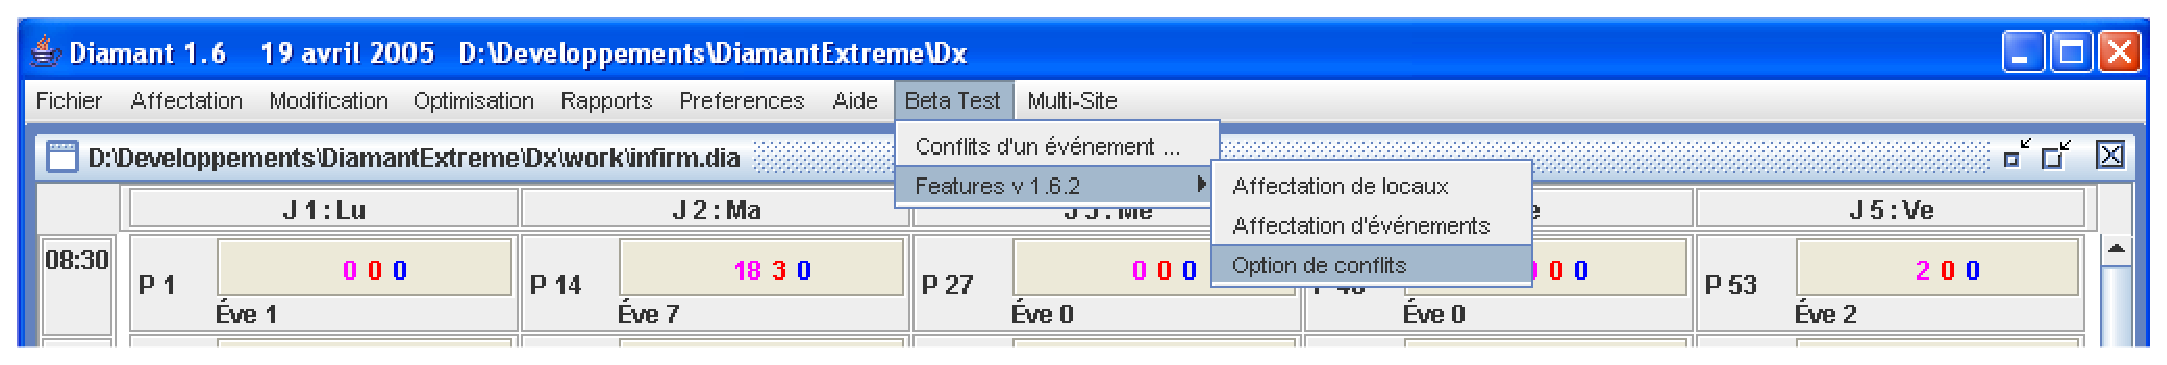
\includegraphics[width=6.0in]{SRS/images/menu_feat_1-6-2.eps}
    \caption{Menu des fonctionnalit�s de la version 1.6.2}\label{menu_feat}
  \end{center}
\end{figure*}

    \subsubsection{Le dialogue d'�v�nements }

Le nouveau dialogue d'�v�nements devra int�grer la fonction et
l'�tat du local comme pr�sent� par la figure \ref{dlg_event}.

\begin{figure*}[h]
  % Requires \usepackage{graphicx}
  \begin{center}
    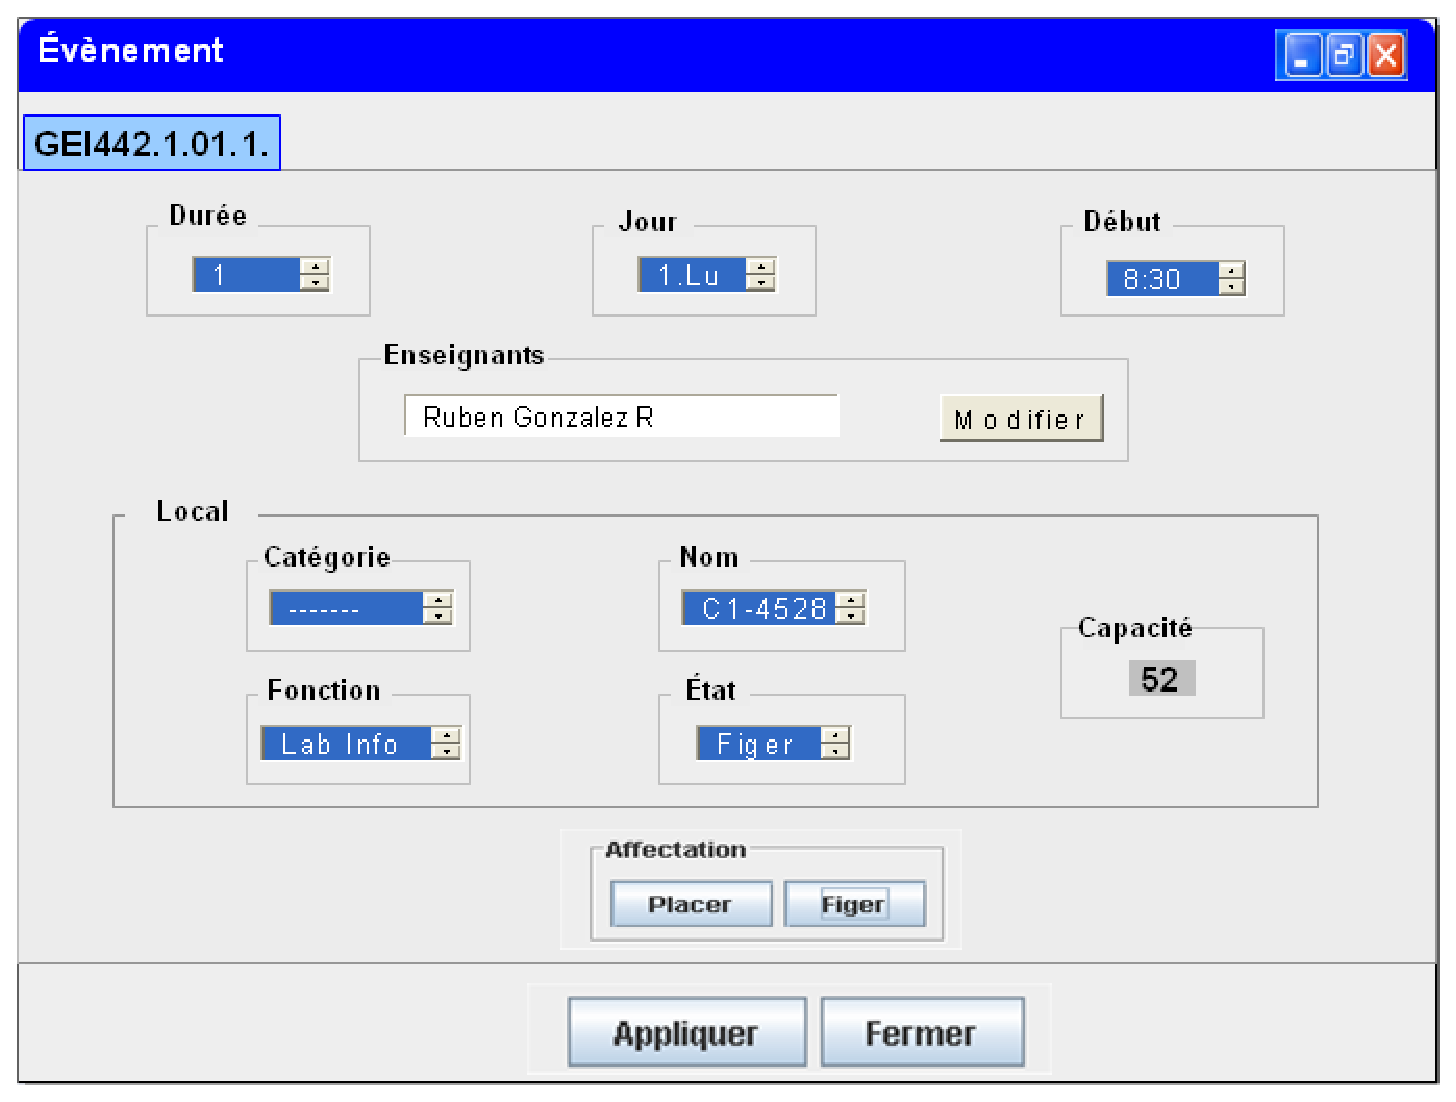
\includegraphics[width=6.0in]{SRS/images/dlg_event.eps}
    \caption{Dialogue d'affectation d'�v�nements de la version 1.6.2}\label{dlg_event}
  \end{center}
\end{figure*}

    \subsubsection{Le dialogue d'option de conflits }

Le nouveau dialogue d'option de conflits devra int�grer un champ
permettant de sp�cifier le taux d'occupation d�sir� pour les
locaux comme pr�sent� par la figure \ref{dlg_conf}.

\begin{figure*}[h]
  % Requires \usepackage{graphicx}
  \begin{center}
    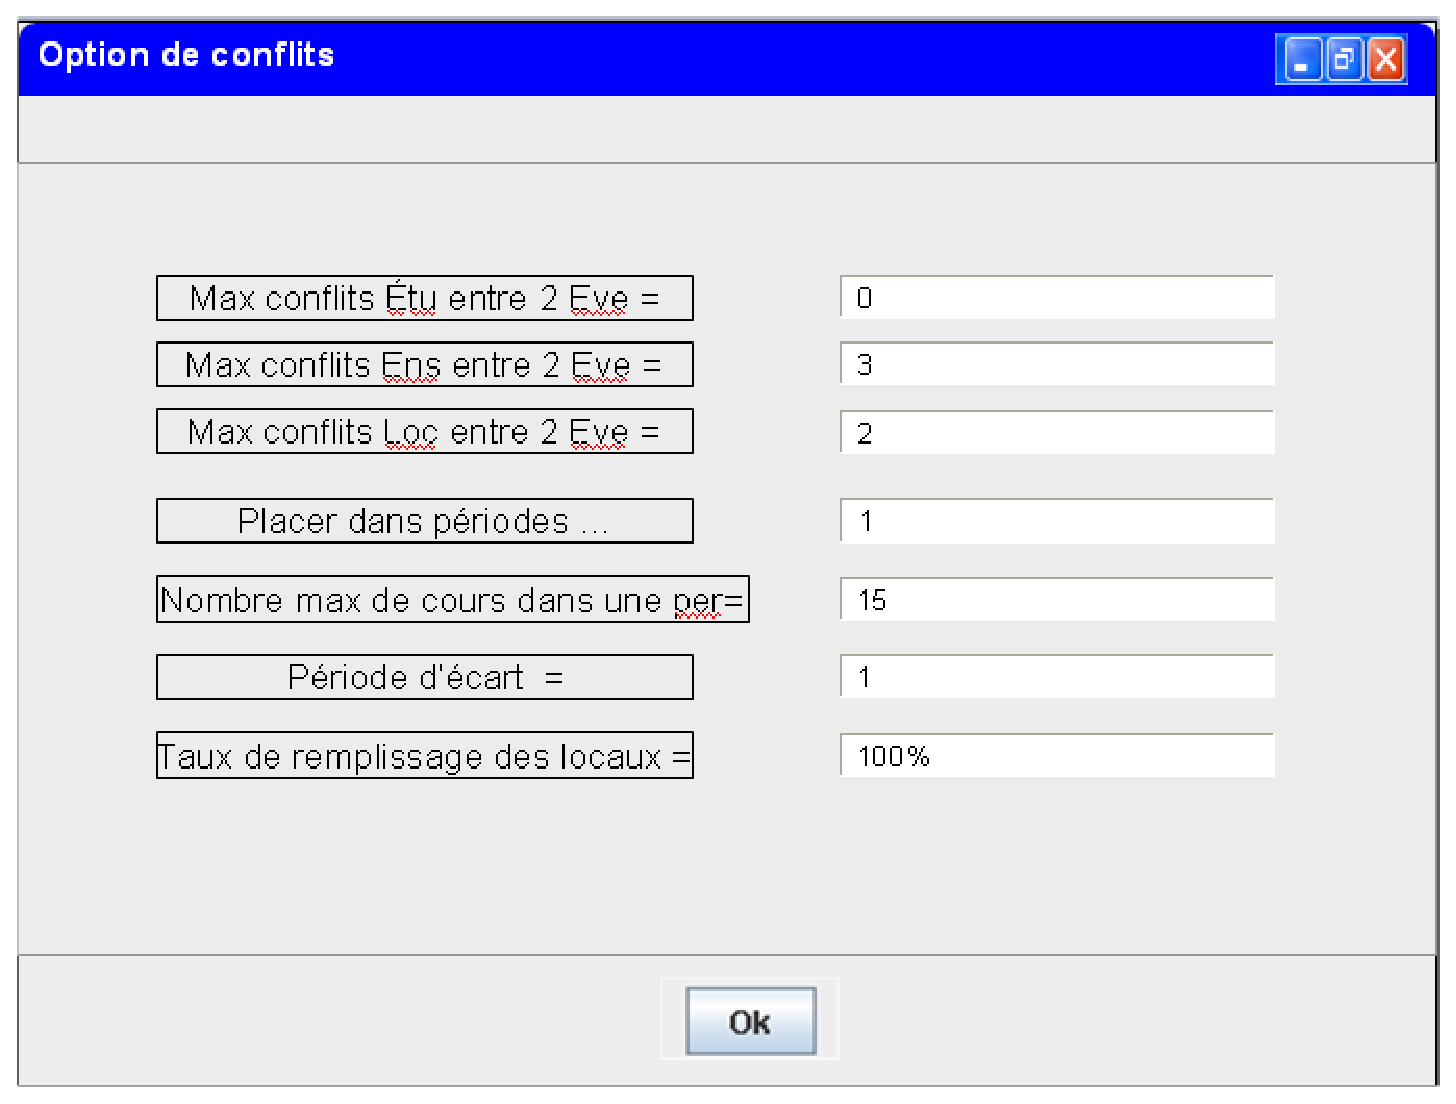
\includegraphics[width=6.0in]{SRS/images/dlg_conflicts.eps}
    \caption{Dialogue d'option de conflits de la version 1.6.2}\label{dlg_conf}
  \end{center}
\end{figure*}

    \subsubsection{Refactoring des �v�nements}

    �tant donn� que les �v�nements devront int�grer de nouveaux
    champs (fonction et �tat), il sera necessaire d'effectuer les t�ches suivantes:

    \begin{itemize}
        \item Refactoring de l'ensemble des �v�nements afin
        d'int�grer les champs fonction et �tat du local dans un
        �v�nement.
        \item Refactoring de l'ensemble des activit�s afin de permettre, d'une part, l'int�gration des champs fonction et �tat du local, et d'autre part,
        la lecture et la sauvegarde des nouveaux champs.
        \item Cr�ation d'un nouvel ensemble contenant la liste des fonctions de locaux
    disponibles.
    \end{itemize}

    \subsubsection{Refactoring des pr�f�rences}
Faire le refactoring des pr�f�rences afin d'y int�grer le nouveau
champ (taux de remplissage des locaux).

    \subsection{Requis fonctionnels}

    De nombreux attributs doivent �tre pris en compte dans cette
affectation.

\subsubsection{Attributs des �v�nements }
\begin{itemize}
    \item Le nom de l'�v�nement: l'identifiant unique de
    l'�v�nement.
    \item L'horaire: la ou les p�riodes dans lesquelles
    l'�v�nement est plac�.
    \item Le nombre d'�tudiants participant � l'�v�nement.
    \item L'identifiant du local associ�.
\end{itemize}

\subsubsection{Attributs des locaux }
\begin{itemize}
    \item Le nom du local: l'identifiant unique du local.
    \item La capacit� du local: nombre de si�ges disponibles dans
    le local.
    \item La cat�gorie du local.
    \item La fonction du local.
    \item L'�tat du local: le local est figer dans une p�riode et par cons�quent il ne
    peut plus faire l'objet d'une affectation.
\end{itemize}

\subsubsection{Contraintes d'optimisation }
\begin{itemize}
    \item Faire une affectation en tenant compte du taux de remplissage des locaux.
    \item Faire une affectation en tenant compte de la
    cat�gorie et de la fonction des locaux.
    \item Faire une affectation en tenant compte de la
    capacit� des locaux.
    \item Assigner un nouveau local � un �v�nement si et seulement
    si cet �v�nement n'est fig� dans aucun local (�tat fig� du
    local).
    \item L'algorithme devra assigner des locaux aux �v�nements plac�s dans
chaque p�riode de la grille.
    \item  L'algorithme devra faire une
assignation de sorte � avoir le maximum d'�tudiants d'un �v�nement
donn� dans le plus petit local disponible.
\end{itemize}

\subsubsection{Sp�cification de l'algorithme d'affectation de locaux}

L'affectation de locaux est un probl�me d'optimisation, dans
lequel on cherche � construire une solution � un probl�me qui
optimise une fonction objectif.

Ce probl�me d'optimisation peut se poser comme suit:

\begin{enumerate}
    \item pour une instance I (par exemple: les horaires des cours �
assurer, des locaux � affecter),
    \item trouver une solution (par exemple une affectation de local �
chaque cours),
    \item qui v�rifie les contraintes (par exemple, il n'y a pas deux
cours en m�me temps dans un local..., le nombre d'�tudiants
suivant un cours est < ou = � la capacit� du local dans lequel ce
cours va se donner),
  \item et qui optimise une fonction objectif (par exemple, minimise
le nombre de locaux).
\end{enumerate}


Pour r�soudre ce probl�me d'optimisation, nous utiliserons la
m�thode gloutonne (algorithme glouton - greedy algorithm) en
construisant tout simplement la solution incr�mentalement, en
rajoutant � chaque pas un �l�ment selon un crit�re glouton, c'est
� dire celui qui nous para�t �localement� le meilleurun choix �
�court terme�.

\begin{description}
    \item[Le probl�me: ] On est dans le cadre de probl�mes d'optimisation.
Plus pr�cis�ment, on est le plus souvent dans le cas suivant:
\begin{itemize}
    \item On a un ensemble fini d'�l�ments, E.
    \item Une solution � notre probl�me est construite � partir des
�l�ments de E: c'est par exemple une partie de E ou un
multi-ensemble d'�l�ments de E ou une suite (finie) d'�l�ments de
E ou une permutation de E qui satisfait une certaine contrainte.
    \item A chaque solution S est associ�e une fonction objectif v(S):
on cherche donc une solution qui maximise (ou minimise) cette
fonction objectif.
\end{itemize}
    \item[Le sch�ma de la m�thode: ] Il est bas� sur un crit�re local de s�lection des �l�ments de E pour
construire une solution optimale. En fait, on travaille sur
l'objet " solution partielle"- "d�but de solution"- et on doit
disposer de:
\begin{itemize}
    \item select: qui choisit le meilleur �l�ment restant selon le crit�re glouton.
    \item complete? qui teste si une solution partielle est une solution (compl�te).
    \item ajoutPossible? qui teste si un �l�ment peut �tre ajout� � une solution partielle, i.e. si la solution partielle
reste un d�but de solution possible apr�s l'ajout de l'�l�ment.
Dans certains cas, c'est toujours vrai!
    \item ajout qui permet d'ajouter un �l�ment � une solution si c'est possible.
\end{itemize}
    \item[L'algorithme est alors: ]

    \begin{verbatim}
    //on va construire la solution dans Sol
    //initialisation
    Ens=E;
    Sol.Init //= ensemble (ou suite) "vide" ou..
    tant que Non Sol.Complete?() ( et Ens.NonVide?())
    select(x,Ens); //on choisit x selon crit�re glouton
    si Sol.AjoutPossible(x) alors Sol.Ajout(x); fsi;
    //dans certains probl�mes, c'est toujours le cas
    si CertainesConditions alors Ens.Retirer(x);
    //selon les cas, x ne sera consid�r� qu'une fois
    // ou jusqu'� qu'il ne puisse plus etre ajout�
    fin tant que;
    //la Solution partielle est compl�te ...normalement
    retourne Sol
    \end{verbatim}
\end{description}

\chapter{Requis des interfaces externes (``External Interface Requirements'')}

According to Richard Thayer (2002), "External interface requirements
specify hardware, software, or database elements with which a system
or component must interface...." This section provides information to
ensure that the system will communicate properly with external
components. If different portions of the product have different
external interfaces, incorporate an instance of this section within
the detailed requirements for each such portion.

Reaching agreement on external and internal system interfaces has been
identified as a software industry best practice (Brown 1996). Place
detailed descriptions of the data and control components of the
interfaces in the data dictionary. A complex system with multiple
subcomponents should use a separate interface specification or system
architecture specification (Hooks and Farry 2001). The interface
documentation could incorporate material from other documents by
reference. For instance, it could point to a separate application
programming interface (API) specification or to a hardware device
manual that lists the error codes that the device could send to the
software.

    \section{Interfaces utilisateurs (``User Interfaces'')}

    Describe the logical characteristics of each user interface that
    the system needs. Some possible items to include are

    \begin{itemize}
        \item References to GUI standards or product family style
              guides that are to be followed.
        \item Standards for fonts, icons, button labels, images, color
              schemes, field tabbing sequences, commonly used
              controls, and the like.
        \item Screen layout or resolution constraints.
        \item Standard buttons, functions, or navigation links that
              will appear on every screen, such as a help button.
        \item Shortcut keys.
        \item Message display conventions.
        \item Layout standards to facilitate software localization.
        \item Accommodations for visually impaired users.
    \end{itemize}

    Document the user interface design details, such as specific
    dialog box layouts, in a separate user interface specification,
    not in the SRS. Including screen mock-ups in the SRS to
    communicate another view of the requirements is helpful, but make
    it clear that the mock-ups are not the committed screen
    designs. If the SRS is specifying an enhancement to an existing
    system, it sometimes makes sense to include screen displays
    exactly as they are to be implemented. The developers are already
    constrained by the current reality of the existing system, so it's
    possible to know up front just what the modified, and perhaps the
    new, screens should look like.

    \section{Interfaces mat�riels (``Hardware Interfaces'')}

    Describe the characteristics of each interface between the
    software and hardware components of the system. This description
    might include the supported device types, the data and control
    interactions between the software and the hardware, and the
    communication protocols to be used.

    \section{Interfaces logiciels (``Software Interfaces'')}

    Describe the connections between this product and other software
    components (identified by name and version), including databases,
    operating systems, tools, libraries, and integrated commercial
    components. State the purpose of the messages, data, and control
    items exchanged between the software components. Describe the
    services needed by external software components and the nature of
    the intercomponent communications. Identify data that will be
    shared across software components. If the data-sharing mechanism
    must be implemented in a specific way, such as a global data area,
    specify this as a constraint.

    \section{Interfaces de communication (``Communications Interfaces'')}

    State the requirements for any communication functions the product
    will use, including e-mail, Web browser, network communications
    protocols, and electronic forms. Define any pertinent message
    formatting. Specify communication security or encryption issues,
    data transfer rates, and synchronization mechanisms. 
\chapter{Autres requis non fonctionnels (``Other Nonfunctional Requirements'')}

This section specifies nonfunctional requirements other than external
interface requirements, which appear in section 4, and constraints,
recorded in section 2.5.

    \section{Requis de performance (``Performance Requirements'')}

    State specific performance requirements for various system
    operations. Explain their rationale to guide the developers in
    making appropriate design choices. For instance, stringent
    database response time demands might lead the designers to mirror
    the database in multiple geographical locations or to denormalize
    relational database tables for faster query responses. Specify the
    number of transactions per second to be supported, response times,
    computational accuracy, and timing relationships for real-time
    systems. You could also specify memory and disk space
    requirements, concurrent user loads, or the maximum number of rows
    stored in database tables. If different functional requirements or
    features have different performance requirements, it's appropriate
    to specify those performance goals right with the corresponding
    functional requirements, rather than collecting them all in this
    one section.

    Quantify the performance requirements as specifically as
    possible--for example, "95 percent of catalog database queries
    shall be completed within 3 seconds on a single-user 1.1-GHz Intel
    Pentium 4 PC running Microsoft Windows XP with at least 60 percent
    of the system resources free." An excellent method for precisely
    specifying performance requirements is Tom Gilb's Planguage,
    described in Chapter 12, "Beyond Functionality: Software Quality
    Attributes."

    \section{Requis face aux dangers et � la sant� (``Safety Requirements'')}

    Safety and security are examples of quality attributes, which are
    more fully addressed in section 5.4. I've called these two
    attributes out in separate sections of the SRS template because if
    they are important at all, they are usually critical. In this
    section, specify those requirements that are concerned with
    possible loss, damage, or harm that could result from the use of
    the product (Leveson 1995). Define any safeguards or actions that
    must be taken, as well as potentially dangerous actions that must
    be prevented. Identify any safety certifications, policies, or
    regulations to which the product must conform. Examples of safety
    requirements are

    \begin{itemize}
        \item{\textbf{SA-1}} The system shall terminate any operation
              within 1 second if the measured tank pressure exceeds 95
              percent of the specified maximum pressure.
        \item{\textbf{SA-2}} The radiation beam shield shall remain
              open only through continuous computer control. The
              shield shall automatically fall into place if computer
              control is lost for any reason.
    \end{itemize}

    \section{Requis au niveau de la s�curit� (``Security Requirements'')}

    Specify any requirements regarding security, integrity, or privacy
    issues that affect access to the product, use of the product, and
    protection of data that the product uses or creates. Security
    requirements normally originate in business rules, so identify any
    security or privacy policies or regulations to which the product
    must conform. Alternatively, you could address these requirements
    through the quality attribute called integrity. Following are
    sample security requirements:

    \begin{itemize}
        \item{\textbf{SE-1}} Every user must change his initially
              assigned login password immediately after his first
              successful login. The initial password may never be
              reused.
        \item{\textbf{SE-2}} A door unlock that results from a
              successful security badge read shall keep the door
              unlocked for 8.0 seconds.
    \end{itemize}

    \section{Attributs de qualit� du logiciel (``Software Quality Attributes'')}

    State any additional product quality characteristics that will be
    important to either customers or developers. (See Chapter 12.)
    These characteristics should be specific, quantitative, and
    verifiable. Indicate the relative priorities of various
    attributes, such as ease of use over ease of learning, or
    portability over efficiency. A rich specification notation such as
    Planguage clarifies the needed levels of each quality much better
    than can simple descriptive statements. 
\chapter{Autres requis (``Other Requirements'')}

Define any other requirements that are not covered elsewhere in the
SRS. Examples include internationalization requirements (currency,
date formatting, language, international regulations, and cultural and
political issues) and legal requirements. You could also add sections
on operations, administration, and maintenance to cover requirements
for product installation, configuration, startup and shutdown,
recovery and fault tolerance, and logging and monitoring
operations. Add any new sections to the template that are pertinent to
your project. Omit this section if all your requirements are
accommodated in other sections.

\chapter{Appendice A: Glossaire (``Appendix A: Glossary'')}

Define any specialized terms that a reader needs to know to properly
interpret the SRS, including acronyms and abbreviations. Spell out
each acronym and provide its definition. Consider building an
enterprise-level glossary that spans multiple projects. Each SRS would
then define only those terms that are specific to an individual
project.

\chapter{Appendice B: Mod�les analytiques (``Appendix B: Analysis Models'')}

This optional section includes or points to pertinent analysis models
such as data flow diagrams, class diagrams, state-transition diagrams,
or entity-relationship diagrams. (See Chapter 11, "A Picture Is Worth
1024 Words.")

\chapter{Appendice C: Liste de points litigieux (``Appendix C: Issue List'')}

This is a dynamic list of the open requirements issues that remain to
be resolved. Issues could include items flagged as TBD, pending
decisions, information that is needed, conflicts awaiting resolution,
and the like. This doesn't necessarily have to be part of the SRS, but
some organizations always attach a TBD list to the SRS. Actively
manage these issues to closure so that they don't impede the timely
baselining of a high-quality SRS.




%\appendix
%\chapter{Description des champs pour \diamant{} 1.5}\label{fields}

\begin{table}[h]
    \begin{tabular}{*{5}{|c}|} \hline
           \itshape Champ & \itshape �l�ment Diamant & \itshape  Description& \itshape Type \footnotemark[1] & \itshape Genre \footnotemark[2]\\ \hline
          Nom du local & Liste de locaux & - & A & \\ \cline{1-4}
          & Liste de locaux & - & A & \\ \cline{2-4}
          & Conflit de capa de locaux & Recalculer les conflits & C & \\ \cline{2-4}
          \raisebox{3.0ex}[1pt]{Capacit�} & P�riode & Rafra�chissement de la p�riode & C & \\ \cline{1-4}
          & Liste de locaux & - & A & \\ \cline{2-4}
          &  & V�rifier si les caract�ristiques & & \\
          &  & du local sont adapt�es & & \\
          \raisebox{4.5ex}[1pt]{Liste de} & \raisebox{3.0ex}[1pt]{Warning de locaux} & � la nature du cours & \raisebox{3.0ex}[1pt]{C} &  \\ \cline{2-4}
          \raisebox{4.5ex}[1pt]{caract�ristiques} & P�riode & Rafra�chissement de la p�riode & C & \raisebox{12.0ex}[1pt]{D} \\ \hline
    \end{tabular}
    \caption{\emph{Fichier de locaux} }
    \label{tableLocaux}
\end{table}
\footnotetext[1]{A: champs affect� - C: champs calcul�} \footnotetext[2]{S: champs statique (immuable) - D: champs dynamique (modifiable)}

\begin{table}[h]
    \begin{tabular}{*{5}{|c}|} \hline
          \itshape Champ & \itshape �l�ment Diamant & \itshape Description & \itshape Type \footnotemark[1] & \itshape Genre \footnotemark[2]\\ \hline
          Instructeur ID(nom) & Liste de professeurs & - & A & S \\ \hline
          & Liste de disp. de profs. & - & A & \\ \cline{2-4}
          & Conflit de disp. de profs. & Recalculer les conflits & C & \\ \cline{2-4}
          \raisebox{3.0ex}[1pt]{Disponibilit�} & P�riode & Rafra�chissement de p�riode & C & \raisebox{3.0ex}[1pt]{D} \\\hline
    \end{tabular}
    \caption{\emph{Fichier de Enseignants}}
    \label{tableEnseignants}
\end{table}

\begin{table}[h]
    \begin{tabular}{*{5}{|c}|} \hline
          \itshape Champ & \itshape �l�ment Diamant & \itshape Description & \itshape Type \footnotemark[1] & \itshape Genre \footnotemark[2]\\ \hline
          Matricule & & - & & S \\ \cline{1-1} \cline{3-3} \cline{5-5}
          Nom et pr�nom & & - & & S \\ \cline{1-1} \cline{3-3} \cline{5-5}
          Sexe & & - & & D \\ \cline{1-1} \cline{3-3} \cline{5-5}
          �tat & \raisebox{4.0ex}[1pt]{Liste d'�tudiants} & - & \raisebox{4.0ex}[1pt]{A} & D \\ \hline
          �tudiant.Activit�ID & & - & & \\ \cline{1-1} \cline{3-3}
          �tudiant.Activit�Nature & \raisebox{1.0ex}[1pt]{Conflits d'�tudiants et} & - & &  \\ \cline{1-1} \cline{3-3}
          �tudiant.Num�roGroupe & \raisebox{1.0ex}[1pt]{Conflits de capacit� de locaux} & - & \raisebox{3.0ex}[1pt]{C} & \raisebox{3.0ex}[1pt]{D} \\ \cline{1-1} \hline
    \end{tabular}
    \caption{\emph{Fichier d'�tudiants}}
    \label{tableEtudiants}
\end{table}


\begin{table}[h]
    \begin{tabular}{*{5}{|c}|} \hline
          \itshape Champ & \itshape �l�ment Diamant & \itshape Description & \itshape Type & \itshape Genre\\ \hline \hline
          Nom d'activit� & Liste d'activit�s & - & A & S \\ \hline
          & Liste d'activit�s & - & A & \\ \cline{2-4}
          & Conflits de locaux & Recalculer les conflits & & \\ \cline{2-2}
          & Conflits de disp. de profs. & si les activit�s sont d�j� & & \\ \cline{2-2}
          \raisebox{4.5ex}[1pt]{Include} & Conflit d'�tudiants & plac�es dans la grille & \raisebox{3.0ex}[1pt]{C} & \raisebox{4.5ex}[1pt]{D} \\ \hline
          Session & Liste d'activit�s & - & A & D \\ \hline
          & Liste de sous-activit�s & - & A & \\ \cline{2-4}
          & Liste d'activit�s & - & A & \\ \cline{2-4}
          & & Dans le cas o� il y a eu un & & \\
          & \raisebox{1.5ex}[1pt]{Warning de locaux} & changement de nature & \raisebox{1.5ex}[1pt]{C} & \\ \cline{2-4}
          & & Dans le cas o� il y a eu une & & \\
          \raisebox{7.0ex}[1pt]{Sous-Activit�.Nature} & \raisebox{1.5ex}[1pt]{Tous les conflits} & insertion/suppression de nature & \raisebox{1.5ex}[1pt]{C} & \raisebox{7.5ex}[1pt]{D} \\ \hline
          & Liste de groupes & - & & \\ \cline{2-3}
          & Liste de sous-activit�s & - & & \\ \cline{2-3}
          & Liste d'activit�s & - & \raisebox{3.0ex}[1pt]{A} &  \\ \cline{2-4}
          & & Dans le cas o� il y a eu une & & \\
          \raisebox{6.0ex}[1pt]{Groupe.Num�ro} & \raisebox{1.5ex}[1pt]{Tous les conflits} & suppression de groupe & \raisebox{1.5ex}[1pt]{C} & \raisebox{6.0ex}[1pt]{S} \\ \hline
          & Liste de bloques & - & & \\ \cline{2-3}
          & Liste de groupes & - & & \\ \cline{2-3}
          & Liste de sous-activit�s & - & & \\ \cline{2-3}
          & Liste d'activit�s & - & \raisebox{4.5ex}[1pt]{A} &  \\ \cline{2-4}
          & & Dans le cas o� il y a eu une & & \\
          \raisebox{6.0ex}[1pt]{Bloque.Num�ro} & \raisebox{1.5ex}[1pt]{Tous les conflits} & suppression de bloque & \raisebox{1.5ex}[1pt]{C} & \raisebox{7.5ex}[1pt]{S} \\ \hline
          & Toutes les listes & - & A & \\ \cline{2-4}
          & Conflit de locaux & - & C & \\ \cline{2-4}
          \raisebox{3.0ex}[1pt]{Bloque.LocalID} & Warning de locaux & - & C & \raisebox{3.0ex}[1pt]{D} \\ \hline
          & Toutes les listes & - & A & \\ \cline{2-4}
          \raisebox{1.5ex}[1pt]{Bloque.P�riodeID} & Tous les conflits & - & C & \raisebox{1.5ex}[1pt]{D} \\ \hline
          & Toutes les listes & - & A & \\ \cline{2-4}
          \raisebox{1.5ex}[1pt]{Bloque.Dure�} & Tous les conflits & - & C & \raisebox{1.5ex}[1pt]{D} \\ \hline
          & Toutes les listes & - & A & \\ \cline{2-4}
          \raisebox{1.5ex}[1pt]{Bloque.Activit�Type} & Warning de locaux & - & C & \raisebox{1.5ex}[1pt]{D} \\ \hline
          & Toutes les listes & - & A & \\ \cline{2-4}
          \raisebox{1.5ex}[1pt]{Bloque.Plac�} & Tous les conflits & - & C & \raisebox{1.5ex}[1pt]{D} \\ \hline
          & Toutes les listes & - & A & \\ \cline{2-4}
          \raisebox{1.5ex}[1pt]{Bloque.Fig�} & Tous les conflits & - & C & \raisebox{1.5ex}[1pt]{D} \\ \hline
          & Toutes les listes & - & A & \\ \cline{2-4}
          \raisebox{1.5ex}[1pt]{Bloque.Instructeur} & Conflit d'instructeur & - & C & \raisebox{1.5ex}[1pt]{D} \\ \hline
    \end{tabular}
    \caption{\emph{Fichier de Cours}}
    \label{tableCours}
\end{table}


  % after \\: \hline or \cline{col0-col2} \cline{col3-col4} .

%\chapter*{Glossaire}

Bla bla bla bla bla.

Bla bla bla bla bla.

%\chapter*{Index}

A
AAA
ABC.

B
Bla bla bla bla bla.

%\include{formules}
\end{articleDX}
\end{document}
